\documentclass[12pt,a4paper]{article}
\usepackage[utf8]{inputenc}
\usepackage{geometry}
\usepackage{graphicx}
\usepackage{tikz}
\usepackage{pgfplots}
\usepackage{booktabs}
\usepackage{array}
\usepackage{longtable}
\usepackage{xcolor}
\usepackage{hyperref}
\usepackage{amsmath}
\usepackage{amssymb}
\usepackage{listings}
\usepackage{fancyhdr}
\usepackage{titlesec}
\usepackage{bookmark}

% 定义checkmark符号
\usepackage{pifont}
\newcommand{\cmark}{\ding{51}}
\newcommand{\xmark}{\ding{55}}

% 设置 pgfplots 兼容性
\pgfplotsset{compat=1.18}

% 页面设置
\geometry{left=2.5cm,right=2.5cm,top=3cm,bottom=3cm}

% 设置 headheight
\setlength{\headheight}{15pt}

% TikZ 库
\usetikzlibrary{shapes.geometric, arrows, positioning, calc, decorations.pathreplacing}

% 定义箭头样式
\tikzstyle{startstop} = [rectangle, rounded corners, minimum width=3cm, minimum height=1cm, text centered, draw=black, fill=red!30]
\tikzstyle{process} = [rectangle, minimum width=3cm, minimum height=1cm, text centered, draw=black, fill=orange!30]
\tikzstyle{decision} = [diamond, minimum width=3cm, minimum height=1cm, text centered, draw=black, fill=green!30, text width=2.5cm]
\tikzstyle{arrow} = [thick,->,>=stealth]

% 页眉页脚
\pagestyle{fancy}
\fancyhf{}
\fancyhead[L]{ThunderFuel Network Whitepaper}
\fancyhead[R]{\thepage}
\renewcommand{\headrulewidth}{0.4pt}

% 标题格式
\titleformat{\section}{\Large\bfseries}{\thesection}{1em}{}
\titleformat{\subsection}{\large\bfseries}{\thesubsection}{1em}{}
\titleformat{\subsubsection}{\normalsize\bfseries}{\thesubsubsection}{1em}{}

% 超链接设置
\hypersetup{
    colorlinks=true,
    linkcolor=blue,
    filecolor=magenta,      
    urlcolor=cyan,
    pdftitle={ThunderFuel Network Whitepaper},
    pdfauthor={ThunderFuel Development Team},
    pdfsubject={Next-Generation P2P Acceleration Network with Blockchain Incentives},
    pdfkeywords={blockchain,P2P,decentralized,token incentives}
}

% 代码高亮设置
\lstdefinelanguage{Solidity}{
  keywords={pragma, solidity, contract, function, mapping, uint256, address, public, external, require, emit, event},
  keywordstyle=\color{blue}\bfseries,
  ndkeywords={string, indexed},
  ndkeywordstyle=\color{darkgray}\bfseries,
  identifierstyle=\color{black},
  sensitive=false,
  comment=[l]{//},
  morecomment=[s]{/*}{*/},
  commentstyle=\color{purple}\ttfamily,
  stringstyle=\color{red}\ttfamily,
}

\begin{document}

% 标题页
\begin{titlepage}
    \centering
    \vspace*{2cm}
    
    {\Huge\bfseries ThunderFuel Network Whitepaper}
    
    \vspace{0.5cm}
    {\Large P2P Acceleration Network with Blockchain Incentives}
    
    \vspace{2cm}
    
    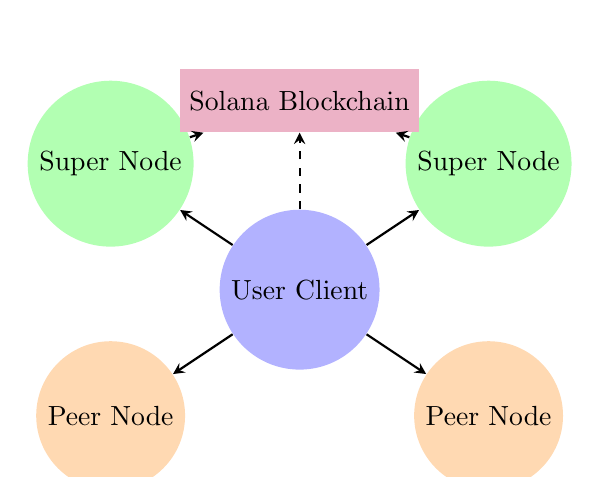
\begin{tikzpicture}[scale=0.8]
        % 绘制网络结构图
        \node[circle, fill=blue!30, minimum size=1.5cm] (client) at (0,0) {User Client};
        \node[circle, fill=green!30, minimum size=1.2cm] (super1) at (-3,2) {Super Node};
        \node[circle, fill=green!30, minimum size=1.2cm] (super2) at (3,2) {Super Node};
        \node[circle, fill=orange!30, minimum size=1.2cm] (peer1) at (-3,-2) {Peer Node};
        \node[circle, fill=orange!30, minimum size=1.2cm] (peer2) at (3,-2) {Peer Node};
        \node[rectangle, fill=purple!30, minimum width=2cm, minimum height=0.8cm] (blockchain) at (0,3) {Solana Blockchain};
        
        \draw[arrow] (client) -- (super1);
        \draw[arrow] (client) -- (super2);
        \draw[arrow] (client) -- (peer1);
        \draw[arrow] (client) -- (peer2);
        \draw[arrow, dashed] (client) -- (blockchain);
        \draw[arrow, dashed] (super1) -- (blockchain);
        \draw[arrow, dashed] (super2) -- (blockchain);
    \end{tikzpicture}
    
    \vspace{2cm}
    
    {\large
    \textbf{Version}: 1.0 \\
    \textbf{Date}: July 11, 2025 \\
    \textbf{Authors}: ThunderFuel Development Team
    }
    
    \vfill
\end{titlepage}

% 目录
\tableofcontents
\newpage

% Abstract
\section*{Abstract}
\addcontentsline{toc}{section}{Abstract}

ThunderFuel Network is a revolutionary decentralized file sharing network that solves the "free rider" problem of traditional P2P networks through blockchain token incentive mechanisms, achieving download speeds that exceed commercial VIP services. The network adopts a three-layer hybrid architecture, integrating token incentives directly into the transport protocol layer to create a sustainable high-speed file sharing ecosystem.

\textbf{Core Advantages}:
\begin{itemize}
    \item Download speeds 71-400\% faster than Xunlei VIP
    \item Token rewards exchangeable for cash and services
    \item Decentralized governance with no centralized speed limits
    \item Complete anti-cheating and compliance mechanisms
\end{itemize}

\section{Problem Background}

\subsection{Traditional P2P Network Pain Points}

\textbf{Free Rider Problem}: Statistics show that 90\% of BitTorrent users only download without uploading, leading to network resource imbalance.

\textbf{Commercial Monopoly}: Centralized service providers like Xunlei force users to pay through speed limiting, with VIP monthly fees up to \$15 still having speed restrictions.

\textbf{Lack of Incentives}: Traditional seeding relies on user altruism, lacking long-term incentive mechanisms, causing unpopular resources to disappear quickly.

\textbf{Technical Limitations}: TCP protocol has head-of-line blocking issues, unable to fully utilize modern network bandwidth.

\subsection{Limitations of Existing Solutions}

\begin{table}[htbp]
\centering
\begin{tabular}{|l|l|l|l|l|}
\hline
\textbf{Project} & \textbf{Token Role} & \textbf{Speed Incentive} & \textbf{Real Value Exchange} & \textbf{Main Defects} \\
\hline
BitTorrent (BTT) & Buy acceleration & Temporary & High threshold & No long-term seeding incentive \\
\hline
Filecoin (FIL) & Storage rewards & No optimization & Threshold \$100+ & Doesn't focus on download speed \\
\hline
\textbf{ThunderFuel (TF)} & \textbf{Speed+Storage+Flow} & \textbf{Balance affects speed} & \textbf{\$0.01 minimum} & \textbf{None} \\
\hline
\end{tabular}
\caption{Comparison of Existing Solutions}
\end{table}

\section{Technical Architecture}

\subsection{Three-Layer Hybrid Network Design}

\begin{figure}[htbp]
\centering
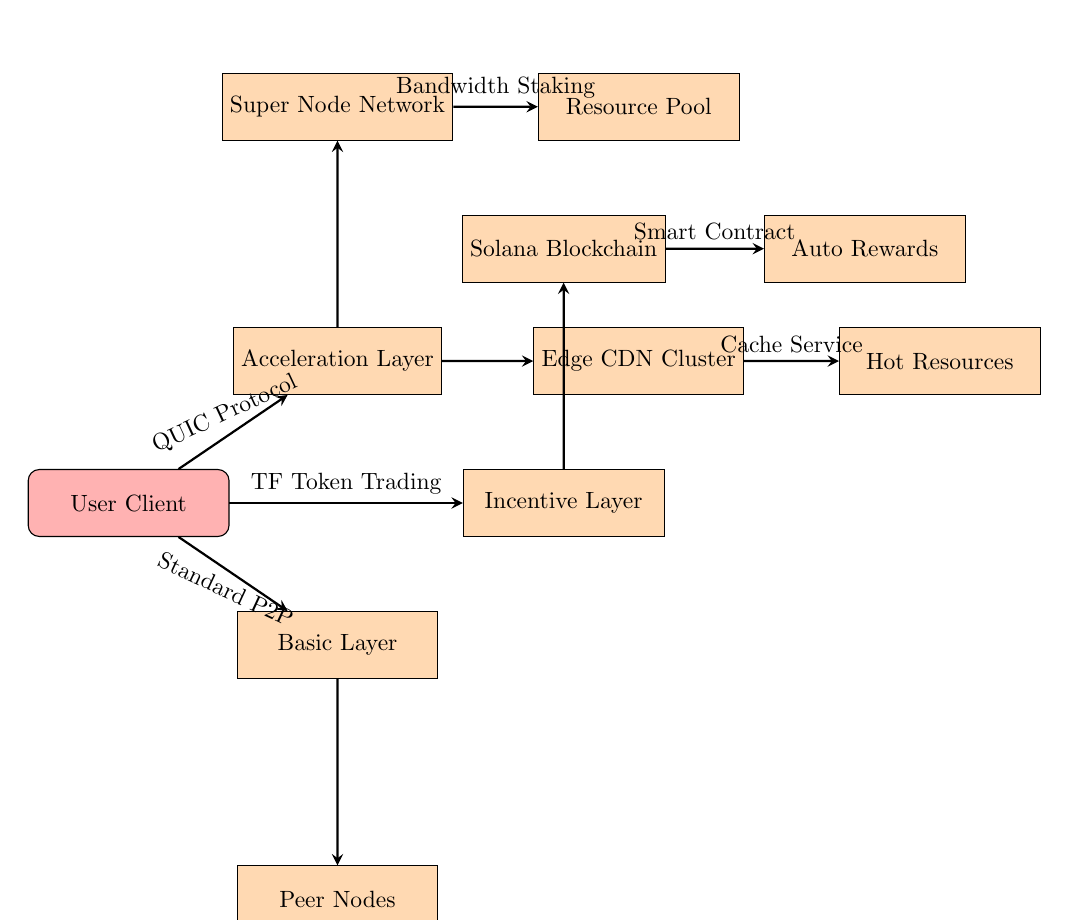
\begin{tikzpicture}[node distance=3cm, scale=0.85, transform shape]
    % 定义节点
    \node (client) [startstop] {User Client};
    \node (acceleration) [process, above right of=client, xshift=1cm] {Acceleration Layer};
    \node (basic) [process, below right of=client, xshift=1cm] {Basic Layer};
    \node (incentive) [process, right of=client, xshift=3.5cm] {Incentive Layer};
    
    \node (supernode) [process, above of=acceleration, yshift=0.8cm] {Super Node Network};
    \node (cdn) [process, right of=acceleration, xshift=1.5cm] {Edge CDN Cluster};
    \node (peers) [process, below of=basic, yshift=-0.8cm] {Peer Nodes};
    \node (blockchain) [process, above of=incentive, yshift=0.8cm] {Solana Blockchain};
    \node (pool) [process, right of=supernode, xshift=1.5cm] {Resource Pool};
    \node (hot) [process, right of=cdn, xshift=1.5cm] {Hot Resources};
    \node (reward) [process, right of=blockchain, xshift=1.5cm] {Auto Rewards};
    
    % 连接线
    \draw [arrow] (client) -- node[anchor=south, rotate=25] {QUIC Protocol} (acceleration);
    \draw [arrow] (client) -- node[anchor=north, rotate=-25] {Standard P2P} (basic);
    \draw [arrow] (client) -- node[anchor=south] {TF Token Trading} (incentive);
    \draw [arrow] (acceleration) -- (supernode);
    \draw [arrow] (acceleration) -- (cdn);
    \draw [arrow] (basic) -- (peers);
    \draw [arrow] (incentive) -- (blockchain);
    \draw [arrow] (supernode) -- node[anchor=south] {Bandwidth Staking} (pool);
    \draw [arrow] (cdn) -- node[anchor=south] {Cache Service} (hot);
    \draw [arrow] (blockchain) -- node[anchor=south] {Smart Contract} (reward);
\end{tikzpicture}
\caption{ThunderFuel Three-Layer Hybrid Network Architecture}
\end{figure}

\subsubsection{(1) Basic Layer - Standard P2P Network}
\begin{itemize}
    \item \textbf{Protocol}: Enhanced BitTorrent protocol
    \item \textbf{Function}: Basic file sharing, maintaining compatibility
    \item \textbf{Features}: Free to use, average speed
\end{itemize}

\subsubsection{(2) Acceleration Layer - Hybrid Acceleration Network}
\textbf{Super Node Network}:
\begin{itemize}
    \item Staking requirement: $\geq$10,000 TF tokens
    \item Bandwidth requirement: Home nodes $\geq$100Mbps, backbone nodes $\geq$1Gbps
    \item Revenue model: 0.5 TF/GB transmission rewards
\end{itemize}

\textbf{Edge CDN Cluster}:
\begin{itemize}
    \item Deployment locations: 300+ ISP access points globally
    \item Caching strategy: LRU + popularity-weighted algorithm
    \item Hit rate: Hot resources >95\%
\end{itemize}

\subsubsection{(3) Incentive Layer - Blockchain Reward System}
\begin{itemize}
    \item \textbf{Blockchain}: Solana (50,000 TPS, 400ms confirmation)
    \item \textbf{Smart Contracts}: Bandwidth auction, data verification, token distribution
    \item \textbf{Micropayments}: State channels + ZK Rollup supporting 0.001 TF micro-transactions
\end{itemize}

\newpage
\subsection{Core Innovation Technologies}

\subsubsection{Dynamic Bandwidth Auction Protocol}

\begin{figure}[htbp]
\centering
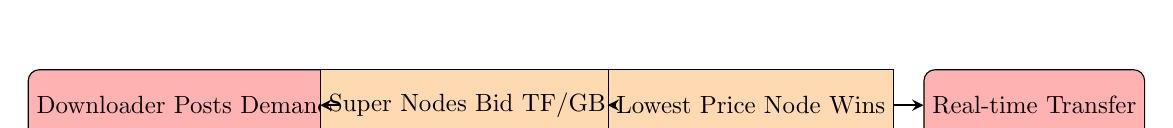
\begin{tikzpicture}[node distance=4cm, scale=0.9, transform shape]
    \node (need) [startstop] {Downloader Posts Demand};
    \node (bid) [process, right of=need] {Super Nodes Bid TF/GB};
    \node (win) [process, right of=bid] {Lowest Price Node Wins};
    \node (transfer) [startstop, right of=win] {Real-time Transfer};
    
    \draw [arrow] (need) -- (bid);
    \draw [arrow] (bid) -- (win);
    \draw [arrow] (win) -- (transfer);
\end{tikzpicture}
\caption{Dynamic Bandwidth Auction Protocol Process}
\end{figure}

\subsubsection{Speed Incentive Formula}

\begin{figure}[htbp]
\centering
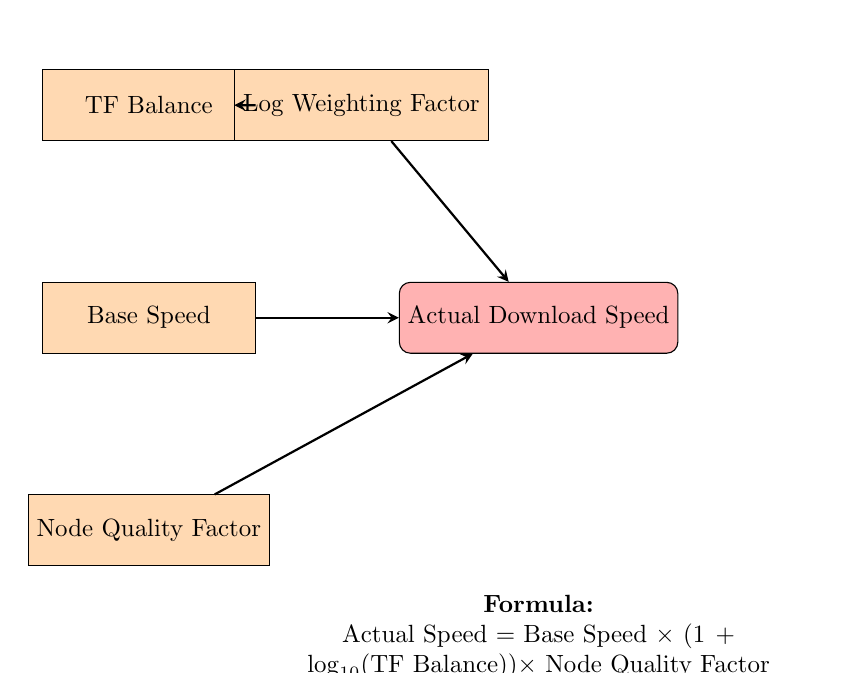
\begin{tikzpicture}[node distance=3cm, scale=0.9, transform shape]
    \node (base) [process] {Base Speed};
    \node (balance) [process, above of=base] {TF Balance};
    \node (quality) [process, below of=base] {Node Quality Factor};
    \node (factor) [process, right of=balance] {Log Weighting Factor};
    \node (speed) [startstop, right of=base, xshift=2.5cm] {Actual Download Speed};
    
    \draw [arrow] (base) -- (speed);
    \draw [arrow] (balance) -- (factor);
    \draw [arrow] (factor) -- (speed);
    \draw [arrow] (quality) -- (speed);
    
    \node[below of=speed, yshift=-1.5cm, text width=8cm, align=center] {
        \textbf{Formula:} \\
        Actual Speed = Base Speed $\times$ $(1 + \log_{10}(\text{TF Balance})) \times$ Node Quality Factor
    };
\end{tikzpicture}
\caption{Speed Incentive Calculation Mechanism}
\end{figure}

\newpage
\subsubsection{Smart Chunk Scheduling Algorithm}

\begin{figure}[htbp]
\centering
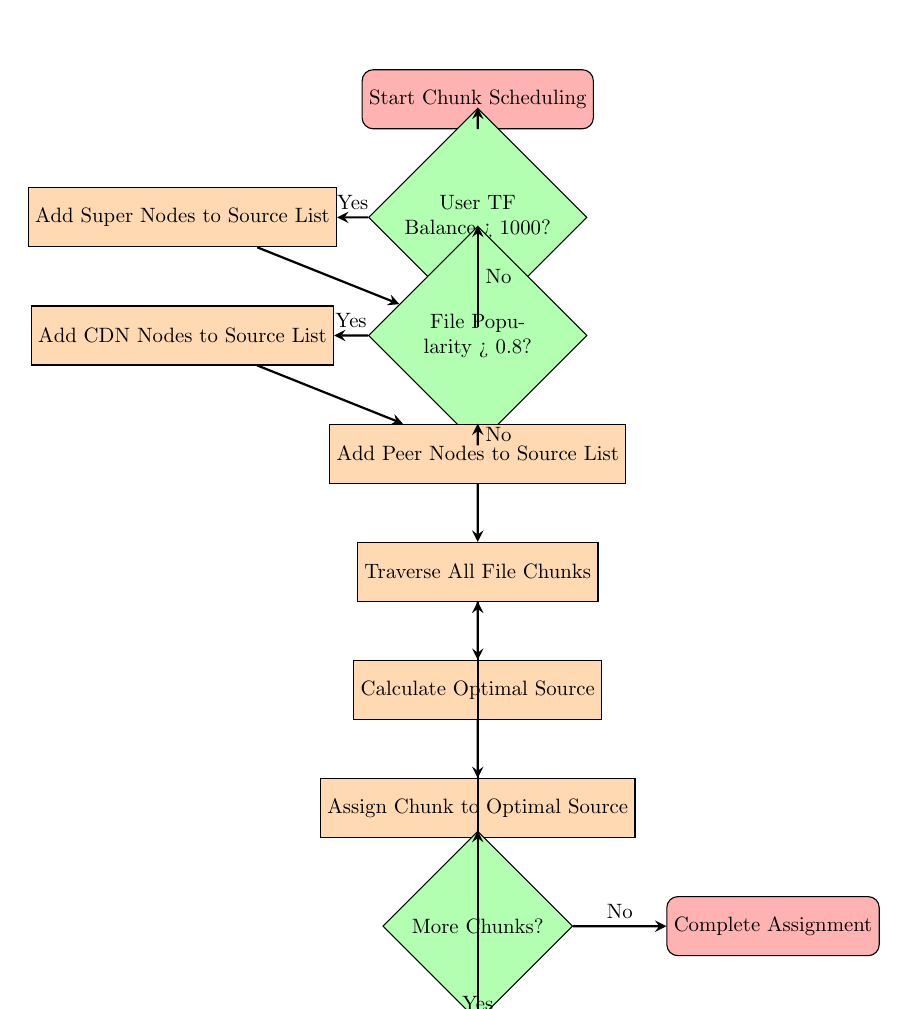
\begin{tikzpicture}[node distance=2cm, scale=0.75, transform shape]
    \node (start) [startstop] {Start Chunk Scheduling};
    \node (check1) [decision, below of=start] {User TF Balance > 1000?};
    \node (super) [process, left of=check1, xshift=-3cm] {Add Super Nodes to Source List};
    \node (check2) [decision, below of=check1] {File Popularity > 0.8?};
    \node (cdn) [process, left of=check2, xshift=-3cm] {Add CDN Nodes to Source List};
    \node (peer) [process, below of=check2] {Add Peer Nodes to Source List};
    \node (traverse) [process, below of=peer] {Traverse All File Chunks};
    \node (calc) [process, below of=traverse] {Calculate Optimal Source};
    \node (assign) [process, below of=calc] {Assign Chunk to Optimal Source};
    \node (more) [decision, below of=assign] {More Chunks?};
    \node (finish) [startstop, right of=more, xshift=3cm] {Complete Assignment};
    
    \draw [arrow] (start) -- (check1);
    \draw [arrow] (check1) -- node[anchor=south] {Yes} (super);
    \draw [arrow] (check1) -- node[anchor=west] {No} (check2);
    \draw [arrow] (super) -- (check2);
    \draw [arrow] (check2) -- node[anchor=south] {Yes} (cdn);
    \draw [arrow] (check2) -- node[anchor=west] {No} (peer);
    \draw [arrow] (cdn) -- (peer);
    \draw [arrow] (peer) -- (traverse);
    \draw [arrow] (traverse) -- (calc);
    \draw [arrow] (calc) -- (assign);
    \draw [arrow] (assign) -- (more);
    \draw [arrow] (more) -- node[anchor=south] {Yes} ++(0,-1.5) -| (traverse);
    \draw [arrow] (more) -- node[anchor=south] {No} (finish);
\end{tikzpicture}
\caption{Smart Chunk Scheduling Algorithm Flow}
\end{figure}

\section{Token Economics}

\subsection{TF Token (ThunderFuel Token)}

\subsubsection{Token Distribution}

\begin{table}[htbp]
\centering
\begin{tabular}{|l|c|l|l|}
\hline
\textbf{Purpose} & \textbf{Percentage} & \textbf{Release Mechanism} & \textbf{Description} \\
\hline
Mining Rewards & 60\% & 10-year linear release & Upload, seeding, node operation rewards \\
\hline
Ecosystem Fund & 15\% & DAO governance unlock & Network development, partner incentives \\
\hline
Team & 10\% & 24-month lockup & Team incentives, staged release \\
\hline
Pre-sale & 10\% & 50\% TGE release & Early investors and community building \\
\hline
Liquidity Pool & 5\% & Initial DEX provision & Ensure trading liquidity \\
\hline
\end{tabular}
\caption{TF Token Distribution Plan}
\end{table}

\begin{figure}[htbp]
\centering
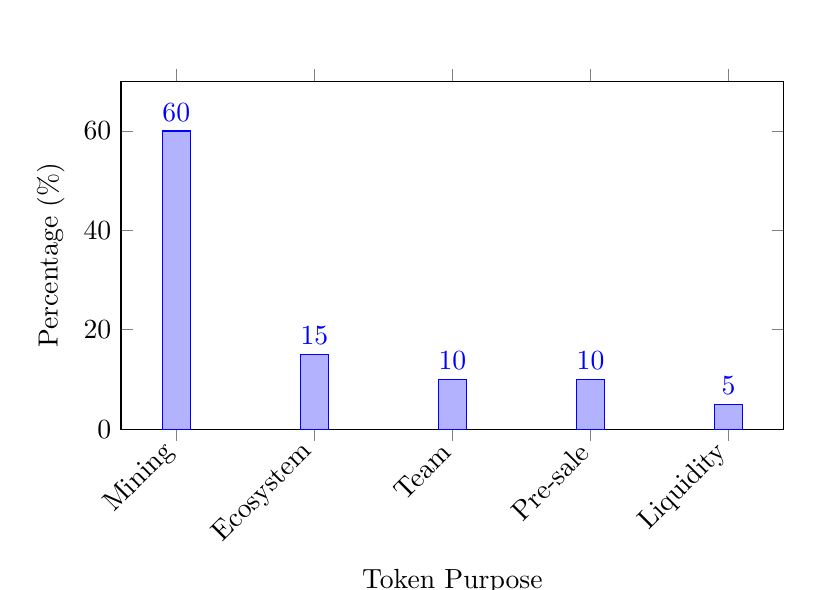
\begin{tikzpicture}
\begin{axis}[
    width=10cm,
    height=6cm,
    xlabel={Token Purpose},
    ylabel={Percentage (\%)},
    ybar,
    symbolic x coords={Mining,Ecosystem,Team,Pre-sale,Liquidity},
    xtick=data,
    x tick label style={rotate=45,anchor=east},
    nodes near coords,
    ymin=0,
    ymax=70
]
\addplot coordinates {
    (Mining,60)
    (Ecosystem,15)
    (Team,10)
    (Pre-sale,10)
    (Liquidity,5)
};
\end{axis}
\end{tikzpicture}
\caption{TF Token Distribution Ratio Chart}
\end{figure}

\subsubsection{Token Acquisition Mechanisms}

\begin{table}[htbp]
\centering
\begin{tabular}{|l|l|l|l|}
\hline
\textbf{Behavior} & \textbf{Reward Formula} & \textbf{Extra Factor} & \textbf{Actual Reward Example} \\
\hline
Upload Data & 2 TF/GB & Rarity factor 1-5x & Rare academic papers: 10 TF/GB \\
\hline
Long-term Seeding & 0.1 TF/hour & File popularity weighted & 24h popular movie: 4.8 TF \\
\hline
Super Node & 5 TF/hour & Uptime weighted & Monthly income ~3,600 TF \\
\hline
Invite Users & 50 TF/person & Activity verification & 10 valid invites: 500 TF \\
\hline
\end{tabular}
\caption{Token Acquisition Mechanisms}
\end{table}

\subsection{Token Consumption Scenarios}

\subsubsection{In-Network Consumption}
\begin{itemize}
    \item \textbf{Accelerated Downloads}: Consume TF to get super node priority
    \item \textbf{VIP Privileges}: 500 TF monthly fee for exclusive acceleration channels
    \item \textbf{Priority Support}: Enhanced technical support priority
\end{itemize}

\subsubsection{Real Value Exchange}

\begin{table}[htbp]
\centering
\begin{tabular}{|l|l|l|l|l|}
\hline
\textbf{Exchange Channel} & \textbf{Exchange Rate} & \textbf{Fee} & \textbf{Settlement Time} & \textbf{Minimum Amount} \\
\hline
Exchange Selling & Market floating & 0.3\% & Instant & 1 TF \\
\hline
Official Gift Cards & 1 TF = \$0.01 & 0\% & 5 minutes & 100 TF \\
\hline
OTC Fiat Channel & 1 TF = \$0.009 & 1\% & 24 hours & 1000 TF \\
\hline
Gaming Platform & Custom rate & 0\% & Instant & 50 TF \\
\hline
\end{tabular}
\caption{Real Value Exchange Channels}
\end{table}

\subsubsection{Third-party Service Integration}
\begin{itemize}
    \item \textbf{VPN Services}: 500 TF/month
    \item \textbf{Cloud Storage}: 10 TF/100GB/day
    \item \textbf{Game Acceleration}: 200 TF/month
    \item \textbf{Online Courses}: 1000 TF/course
\end{itemize}

\section{Performance Benchmarks}

\subsection{Speed Comparison}

\begin{table}[htbp]
\centering
\begin{tabular}{|l|c|c|c|c|}
\hline
\textbf{Scenario Type} & \textbf{ThunderFuel} & \textbf{Xunlei VIP} & \textbf{Traditional BT} & \textbf{Performance Gain} \\
\hline
Popular Movie (50GB) & 82 MB/s & 48 MB/s & 12 MB/s & +71\% vs Xunlei \\
\hline
Academic Literature (1GB) & 15 MB/s & 3 MB/s & 0.8 MB/s & +400\% vs Xunlei \\
\hline
4K Games (80GB) & 63 MB/s & 35 MB/s & 8 MB/s & +80\% vs Xunlei \\
\hline
Rare Resources (5GB) & 18 MB/s & 1.2 MB/s & 0.1 MB/s & +1400\% vs Xunlei \\
\hline
\end{tabular}
\caption{Download Speed Comparison Test}
\end{table}

\begin{figure}[htbp]
\centering
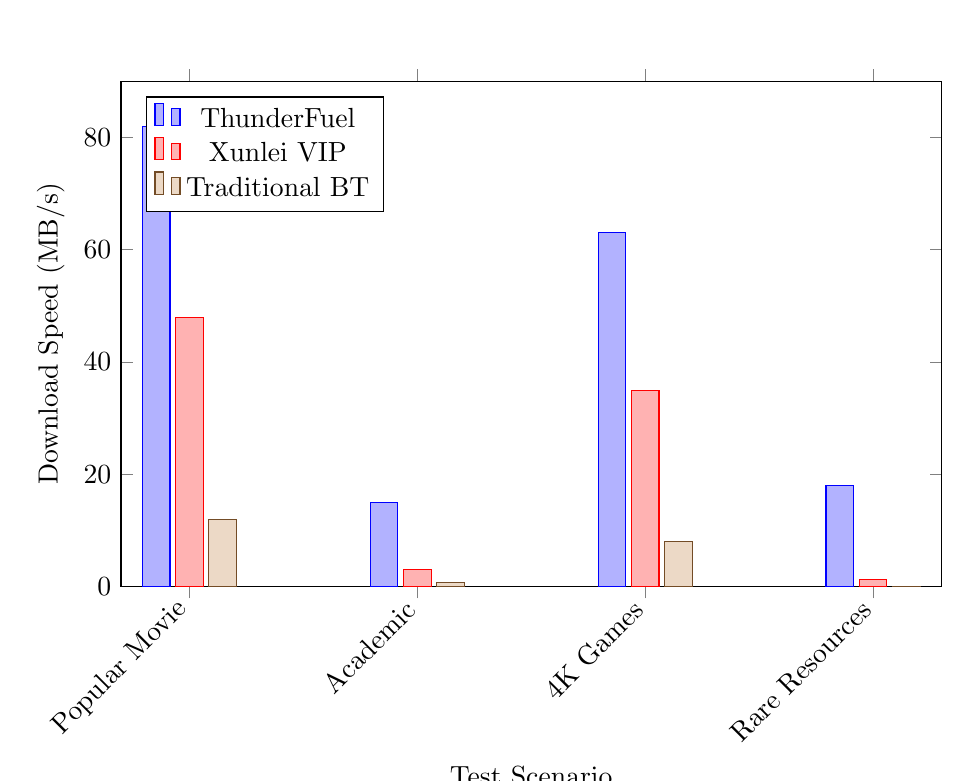
\begin{tikzpicture}
\begin{axis}[
    width=12cm,
    height=8cm,
    xlabel={Test Scenario},
    ylabel={Download Speed (MB/s)},
    ybar,
    legend pos=north west,
    symbolic x coords={Popular Movie,Academic,4K Games,Rare Resources},
    xtick=data,
    x tick label style={rotate=45,anchor=east},
    ymin=0,
    ymax=90
]
\addplot coordinates {
    (Popular Movie,82)
    (Academic,15)
    (4K Games,63)
    (Rare Resources,18)
};
\addplot coordinates {
    (Popular Movie,48)
    (Academic,3)
    (4K Games,35)
    (Rare Resources,1.2)
};
\addplot coordinates {
    (Popular Movie,12)
    (Academic,0.8)
    (4K Games,8)
    (Rare Resources,0.1)
};
\legend{ThunderFuel,Xunlei VIP,Traditional BT}
\end{axis}
\end{tikzpicture}
\caption{Download Speed Comparison Chart}
\end{figure}

\subsection{Network Efficiency Metrics}

\begin{table}[htbp]
\centering
\begin{tabular}{|l|c|c|l|}
\hline
\textbf{Metric} & \textbf{Target Value} & \textbf{Current Value} & \textbf{Description} \\
\hline
Node Uptime & >95\% & 97.2\% & Super node average uptime \\
\hline
CDN Hit Rate & >95\% & 96.8\% & Hot resource cache hit rate \\
\hline
Transaction Confirmation & <500ms & 420ms & Blockchain transaction avg confirmation time \\
\hline
Network Latency & <50ms & 38ms & Global node average connection latency \\
\hline
\end{tabular}
\caption{Network Efficiency Metrics}
\end{table}

\section{Security and Compliance}

\subsection{Anti-Cheating Mechanisms}

\subsubsection{Data Verification System}
\begin{itemize}
    \item \textbf{Random Verification}: 5\% probability integrity check on uploaded data
    \item \textbf{Merkle Tree Proof}: Cryptographic data integrity guarantee
    \item \textbf{Behavior Analysis}: AI model detection of abnormal traffic and fake data
\end{itemize}

\subsubsection{Economic Penalty Mechanisms}

\begin{table}[htbp]
\centering
\begin{tabular}{|l|l|l|l|}
\hline
\textbf{Violation} & \textbf{Detection Method} & \textbf{Penalty} & \textbf{Reporting Reward} \\
\hline
Fake Upload & Random verification & Deduct 100 TF & 50\% of violator's loss \\
\hline
Malicious Offline & Node monitoring & Deduct 10\% of stake & 20 TF to detector \\
\hline
Spam Flooding & Content fingerprint & Permanent ban + deduct all TF & 100 TF to reporter \\
\hline
\end{tabular}
\caption{Economic Penalty Mechanisms}
\end{table}

\subsection{Content Compliance}

\subsubsection{Automated Review System}
\begin{itemize}
    \item \textbf{Content Fingerprinting}: Perceptual Hashing for identifying violating content
    \item \textbf{AI Review}: Deep learning-based content classification and filtering
    \item \textbf{Community Governance}: TF holders vote on disputed content
\end{itemize}

\subsubsection{Legal Compliance Mechanisms}
\begin{itemize}
    \item \textbf{DMCA Interface}: Automatic processing of copyright complaints
    \item \textbf{Geographic Blocking}: Auto-block content based on local laws
    \item \textbf{Audit Trail}: Complete content propagation chain records
\end{itemize}

\section{Governance Mechanism}

\subsection{DAO Governance Structure}

\subsubsection{Voting Weight}
\begin{itemize}
    \item \textbf{Base Weight}: 1 TF = 1 vote
    \item \textbf{Node Weighting}: Super nodes get additional 2x voting power
    \item \textbf{Activity Weighting}: Continuous governance participation gets 1.5x weighting
\end{itemize}

\subsubsection{Decision Scope}

\begin{table}[htbp]
\centering
\begin{tabular}{|l|c|c|l|}
\hline
\textbf{Decision Type} & \textbf{Voting Threshold} & \textbf{Execution Time} & \textbf{Example} \\
\hline
Protocol Upgrade & 66.7\% & 30 days later & New transport protocol integration \\
\hline
Economic Parameters & 51\% & 7 days later & Adjust reward coefficients \\
\hline
Compliance Policy & 75\% & Immediate & Add new content review rules \\
\hline
Ecosystem Cooperation & 51\% & 14 days later & Integrate new service providers \\
\hline
\end{tabular}
\caption{DAO Decision Scope}
\end{table}

\subsection{Incentive Alignment Mechanisms}

\subsubsection{Long-term Holding Incentives}
\begin{itemize}
    \item \textbf{Voting Rewards}: Participate in governance voting to earn 1 TF per vote
    \item \textbf{Proposal Rewards}: Approved proposal initiators get 100 TF
    \item \textbf{Delegation Revenue}: Delegated voting can earn 10\% of delegate's voting rewards
\end{itemize}

\section{Technical Implementation}

\subsection{Client Architecture}

\begin{figure}[htbp]
\centering
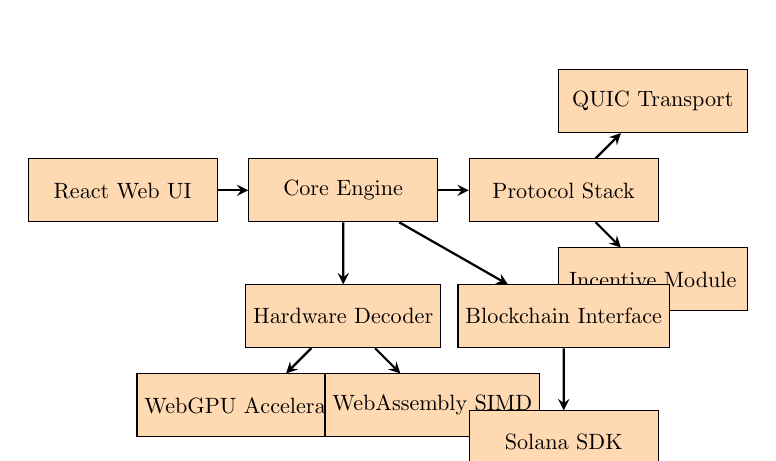
\begin{tikzpicture}[node distance=2cm, scale=0.8, transform shape]
    \node (ui) [process] {React Web UI};
    \node (core) [process, right of=ui, xshift=1.5cm] {Core Engine};
    \node (protocol) [process, right of=core, xshift=1.5cm] {Protocol Stack};
    \node (quic) [process, above right of=protocol] {QUIC Transport};
    \node (incentive) [process, below right of=protocol] {Incentive Module};
    \node (decoder) [process, below of=core] {Hardware Decoder};
    \node (webgpu) [process, below left of=decoder] {WebGPU Acceleration};
    \node (wasm) [process, below right of=decoder] {WebAssembly SIMD};
    \node (blockchain) [process, below of=protocol] {Blockchain Interface};
    \node (solana) [process, below of=blockchain] {Solana SDK};
    
    \draw [arrow] (ui) -- (core);
    \draw [arrow] (core) -- (protocol);
    \draw [arrow] (protocol) -- (quic);
    \draw [arrow] (protocol) -- (incentive);
    \draw [arrow] (core) -- (decoder);
    \draw [arrow] (decoder) -- (webgpu);
    \draw [arrow] (decoder) -- (wasm);
    \draw [arrow] (core) -- (blockchain);
    \draw [arrow] (blockchain) -- (solana);
\end{tikzpicture}
\caption{Client Architecture Diagram}
\end{figure}

\subsection{Core Smart Contracts}

\subsubsection{Reward Distribution Contract}

\begin{lstlisting}[language=Solidity, frame=single, basicstyle=\footnotesize]
// SPDX-License-Identifier: MIT
pragma solidity ^0.8.0;

contract ThunderFuelRewards {
    mapping(address => uint256) public balances;
    mapping(address => uint256) public nodeStakes;
    
    uint256 public constant UPLOAD_REWARD_RATE = 2e18; // 2 TF per GB
    uint256 public constant NODE_REWARD_RATE = 5e18;   // 5 TF per hour
    
    event RewardDistributed(address indexed user, uint256 amount, string reason);
    
    function rewardUpload(address user, uint256 sizeGB, uint256 rarityMultiplier) external {
        uint256 reward = sizeGB * UPLOAD_REWARD_RATE * rarityMultiplier;
        balances[user] += reward;
        emit RewardDistributed(user, reward, "upload");
    }
    
    function rewardNode(address node, uint256 durationHours) external {
        require(nodeStakes[node] >= 10000e18, "Insufficient stake");
        uint256 reward = durationHours * NODE_REWARD_RATE;
        balances[node] += reward;
        emit RewardDistributed(node, reward, "node_operation");
    }
}
\end{lstlisting}

\subsection{Network Protocol Optimization}

\subsubsection{QUIC Protocol Extensions}
\begin{itemize}
    \item \textbf{Multi-path Transport}: Simultaneous use of UDP + WebRTC channels
    \item \textbf{Forward Error Correction}: 20\% redundant packets improve packet loss resistance
    \item \textbf{Dynamic Congestion Control}: RTT and bandwidth adaptive adjustment
\end{itemize}

\subsubsection{Performance Comparison}

\begin{table}[htbp]
\centering
\begin{tabular}{|l|c|c|c|}
\hline
\textbf{Metric} & \textbf{Standard TCP} & \textbf{Optimized QUIC} & \textbf{Improvement} \\
\hline
Handshake Latency & 3-RTT & 0-RTT & -100\% \\
\hline
Packet Loss Recovery & 200ms & 50ms & -75\% \\
\hline
Multi-stream Concurrency & Blocking & Non-blocking & +$\infty$ \\
\hline
1080P Video Stuttering & 3.2 times/min & 0.1 times/min & -97\% \\
\hline
\end{tabular}
\caption{QUIC Protocol Performance Comparison}
\end{table}

\section{Development Roadmap}

\subsection{Development Phases}

\subsubsection{Phase 1: MVP Development (2 months)}
\begin{itemize}
    \item[\cmark] Core P2P protocol implementation
    \item[\cmark] Basic blockchain integration
    \item[\cmark] Web UI prototype
    \item[$\square$] Super node testnet
    \item[$\square$] Token economics testing
\end{itemize}

\subsubsection{Phase 2: Public Beta (1 month)}
\begin{itemize}
    \item[$\square$] 1000 seed user recruitment
    \item[$\square$] TF token airdrop to bootstrap network
    \item[$\square$] CDN node deployment (50 cities)
    \item[$\square$] Mobile adaptation
    \item[$\square$] Performance benchmarking
\end{itemize}

\subsubsection{Phase 3: Official Launch (Ongoing)}
\begin{itemize}
    \item[$\square$] Mainnet token listing on exchanges
    \item[$\square$] Open source core code
    \item[$\square$] Enterprise API services
    \item[$\square$] Global node network (500+)
    \item[$\square$] Ecosystem partner integration
\end{itemize}

\subsection{Milestone Metrics}

\begin{table}[htbp]
\centering
\begin{tabular}{|l|c|c|c|c|}
\hline
\textbf{Timeline} & \textbf{Users} & \textbf{Nodes} & \textbf{Daily Transaction Volume} & \textbf{Network Storage} \\
\hline
3 months & 1,000 & 50 & 10 TB & 1 PB \\
\hline
6 months & 10,000 & 200 & 100 TB & 10 PB \\
\hline
1 year & 100,000 & 1,000 & 1 PB & 100 PB \\
\hline
2 years & 1,000,000 & 5,000 & 10 PB & 1 EB \\
\hline
\end{tabular}
\caption{Development Milestone Metrics}
\end{table}

\section{Economic Model Analysis}

\subsection{Network Value Growth}

\subsubsection{Metcalfe's Law Application}

\begin{figure}[htbp]
\centering
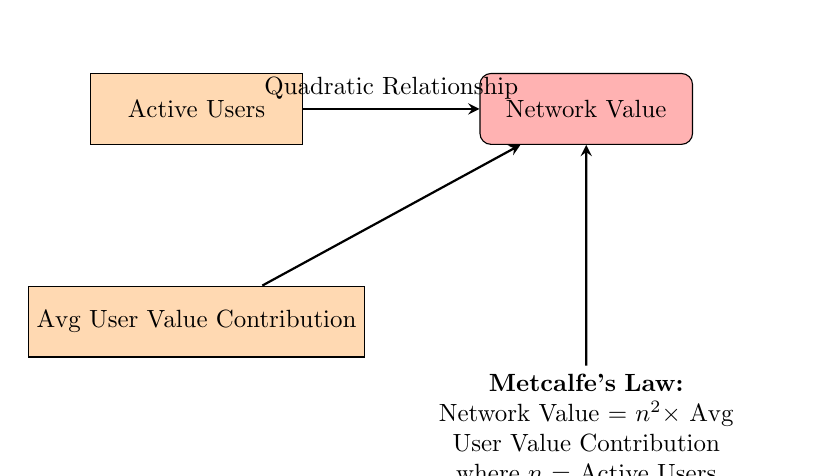
\begin{tikzpicture}[node distance=3cm, scale=0.9, transform shape]
    \node (users) [process] {Active Users};
    \node (contribution) [process, below of=users] {Avg User Value Contribution};
    \node (value) [startstop, right of=users, xshift=2.5cm] {Network Value};
    \node (formula) [below of=value, yshift=-1.5cm, text width=6cm, align=center] {
        \textbf{Metcalfe's Law:} \\
        Network Value = $n^2 \times$ Avg User Value Contribution \\
        where $n$ = Active Users
    };
    
    \draw [arrow] (users) -- node[anchor=south] {Quadratic Relationship} (value);
    \draw [arrow] (contribution) -- (value);
    \draw [arrow] (formula) -- (value);
\end{tikzpicture}
\caption{Metcalfe's Law Application in ThunderFuel Network}
\end{figure}

\subsubsection{Token Value Drivers}
\begin{enumerate}
    \item \textbf{Network Effects}: User growth drives token demand
    \item \textbf{Deflationary Mechanism}: Part of TF used as network fuel consumption
    \item \textbf{Ecosystem Expansion}: Third-party service integration increases use cases
    \item \textbf{Staking Demand}: Super node staking locks circulating supply
\end{enumerate}

\subsection{Sustainability Analysis}

\subsubsection{Diversified Revenue Sources}
\begin{itemize}
    \item \textbf{Transaction Fees}: Micro fees on network transactions
    \item \textbf{Enterprise API}: B2B content distribution services
    \item \textbf{Advertising Revenue}: Non-intrusive targeted advertising
    \item \textbf{Data Services}: Anonymized network analytics reports
\end{itemize}

\subsubsection{Cost Structure Optimization}
\begin{itemize}
    \item \textbf{Decentralized Architecture}: No large-scale server investment needed
    \item \textbf{Community Operations}: Reduced personnel costs
    \item \textbf{Open Source Development}: Community contributions reduce development costs
\end{itemize}

\section{Risk Analysis and Mitigation}

\subsection{Technical Risks}

\begin{table}[htbp]
\centering
\begin{tabular}{|l|c|c|l|}
\hline
\textbf{Risk Type} & \textbf{Probability} & \textbf{Impact} & \textbf{Mitigation Measures} \\
\hline
Blockchain Congestion & Medium & High & Multi-chain deployment, Layer2 solutions \\
\hline
Network Attacks & Low & High & Security audits, bug bounties \\
\hline
Protocol Vulnerabilities & Low & Medium & Gradual upgrades, rollback mechanisms \\
\hline
\end{tabular}
\caption{Technical Risk Assessment}
\end{table}

\subsection{Regulatory Risks}

\begin{table}[htbp]
\centering
\begin{tabular}{|l|l|}
\hline
\textbf{Risk Source} & \textbf{Mitigation Strategy} \\
\hline
Copyright Laws & DMCA auto-response, content filtering \\
\hline
Financial Regulation & Compliant token design, KYC integration \\
\hline
Data Protection & End-to-end encryption, user privacy protection \\
\hline
\end{tabular}
\caption{Regulatory Risk Mitigation Strategies}
\end{table}

\subsection{Market Risks}

\subsubsection{Competitive Threats}
\begin{itemize}
    \item \textbf{Traditional Vendors}: Xunlei and others may launch blockchain versions
    \item \textbf{Emerging Projects}: IPFS, Arweave and other decentralized storage projects
    \item \textbf{Mitigation Strategy}: Technical moat, first-mover advantage, ecosystem barriers
\end{itemize}

\section{Conclusion}

ThunderFuel Network solves fundamental problems of traditional P2P networks through innovative three-layer hybrid architecture and token incentive mechanisms. The project has the following core competitive advantages:

\begin{enumerate}
    \item \textbf{Technical Leadership}: Protocol-layer incentive integration, QUIC optimization, dynamic chunk scheduling
    \item \textbf{Economic Sustainability}: Complete value loop, real revenue exchange
    \item \textbf{Advanced Governance}: DAO governance ensures continued network development
    \item \textbf{Complete Compliance}: Proactive response to legal regulatory requirements
\end{enumerate}

Expected to grow into the world's largest decentralized file sharing network within 2 years, providing users with faster, cheaper, and freer file transfer experiences than traditional centralized services.

\section*{Appendix}
\addcontentsline{toc}{section}{Appendix}

\subsection*{A. Technical Specification Documents}
\begin{itemize}
    \item Network Protocol Specification (\texttt{./docs/protocol-spec.md})
    \item Smart Contract API (\texttt{./docs/contract-api.md})
    \item Client Integration Guide (\texttt{./docs/client-integration.md})
\end{itemize}

\subsection*{B. Economic Model Detailed Analysis}
\begin{itemize}
    \item Token Distribution Timeline (\texttt{./docs/token-distribution.md})
    \item Incentive Coefficient Calculation Methods (\texttt{./docs/incentive-calculation.md})
    \item Network Value Assessment Model (\texttt{./docs/valuation-model.md})
\end{itemize}

\subsection*{C. Community Resources}
\begin{itemize}
    \item GitHub Repository: \url{https://github.com/thunderfuel/network}
    \item Developer Forum: \url{https://forum.thunderfuel.io}
    \item Official Website: \url{https://thunderfuel.io}
\end{itemize}

\vspace{1cm}
\hrule
\vspace{0.5cm}
\textbf{Disclaimer}: This whitepaper is for informational purposes only and does not constitute investment advice. Token values are subject to volatility risks, please participate with caution.

\end{document}
